%
% You may wish to use some of the following options of the iitthesis
% package:
%
% fullpageDraft      avoid the margins necessary for proper binding and
%   just view or print a draft.
% beforeDefense      make the personal acknowledgements invisible;
%   use this to print the copies you submit initially to the grad school
%   for sending to the opponent panel, i.e. thesis readers (who shouldn't
%   see those parts). For the final submission, after having successfully
%   defended - drop this option.
% noabbrevs          avoid generation of a notation & abbreviations list
%
% Additionally, you must specify the degree for which you're writing
% your thesis (MSc/PhD/MArch etc.)
%
\documentclass[MSc,beforeDefense]{misc/iitthesis}


% Definitions of info fields for the thesis - subject, advisor,
% faculty, acknowledgements, etc. etc. The thesis-fields file 
% contains Hebrew text, and should use the UTF-8 character set
% encoding (not iso-8859-8-i or windows codepage 1255).
% This file contains definitions of various fields used
% in various places throughout the thesis (in the title
% pages mostly). Whatever isn't define here has some
% default (and usually irrelevant) text.

\authorEnglish{Shaked Elias-Zada}
\authorHebrew{שקד אליאס-זדה}

\titleEnglish{Quancurrent: \\ A Concurrent Quantiles Sketch}
\titleHebrew{\textenglish{Quancurrent:\\} סקיצה מקבילית לשערוך שברונים של שטף מידע}

\disciplineEnglish{The Andrew and Erna Viterbi Faculty of Electrical and Computer Engineering}
\disciplineHebrew{הפקולטה להנדסת חשמל ומחשבים ע״ש אנדרו וארנה ויטרבי}

\supervisionEnglish{This research was carried out under the supervision of Prof.~Idit Keidar, in the Faculty of Electrical and Computer Engineering.}
\supervisionHebrew{המחקר בוצע בהנחייתו של פרופסור עדית קידר, בפקולטה הנדסת חשמל ומחשבים.}

\GregorianDateEnglish{September 2022}
\GregorianDateHebrew{ספטמבר \textenglish{2022}}
\JewishDateEnglish{Elul, 5782}
\JewishDateHebrew{אלול התשפ״ב}

%\financialAcknowledgementEnglish{The Technion's funding of this research is hereby acknowledged.}
%\financialAcknowledgementHebrew{הכרת תודה מסורה לטכניון על מימון מחקר זה.}

\publicationInfoEnglish{%
%Remove this parenthesized note and the line following it!
% (The grad school guidelines now require that you mention the following regarding publications of your thesis work; but of course, remove this parenthesized note...; you will find the note in the \texttt{thesis-fields.tex} file. The entries for the publication list are BiBTeX bibliography entries, separate from those in the main bibliography: You must place them in \texttt{front/pubinfo.bib}; make sure their labels are distinct from entries in the main bibliography; and order them in the order in which you want them to appear --- they will not be sorted. Note also that the document may need to be processed several times before the list of publications actually appears)

Some results in this thesis have been published as articles by the author and research collaborators in conferences and journals during the course of the author's master research period, the most up-to-date versions of which being:

\butcheredbibliography{front/pubinfo.bib}
}

\publicationInfoHebrew{%
% (התייחסות לפרסומים, שמופיעה להלן, הינה הכרחית לפי תקנות ביה"ס ללימודי מוסמכים; כמובן שיש למחוק את ההערה הזו שבסוגריים... תוכן זה נמצאה בקובץ \textenglish{\texttt{thesis-fields.tex}}. הרשומות לצורך רשימת הפרסומים הינן רשומות \textenglish{BibTeX}, נפרדות מן הרשומות בביבליוגרפיה העיקרית של המסמך: עליך לשים אותן בקובץ \textenglish{\texttt{front/pubinfo.bib}}; הקפיד/י שהתוויות שלהם יהיו שונות מתוויות הרשומות בביליוגרפיה העיקרית. רשום/י אותם בסדר בהם תרצה/י שיופיעו ברשימה --- שכן הן לא ימוינו. כן שים/י לב שייתכן שיהיה צורך להדר את המסמך פעם או פעמיים נוספות עד שהרשימה אכן תופיע כראוי.)

חלק מן התוצאות בחיבור זה פורסמו כמאמרים מאת המחבר ושותפיו למחקר בכנסים ובכתבי-עת במהלך תקופת מחקר המאסטר של המחבר, אשר גרסאותיהם העדכניות ביותר הינן:%

\begin{otherlanguage}{english}%
\butcheredbibliography{front/pubinfo.bib}
\end{otherlanguage}%
}

\addbibresource{back/general.bib}
% \thesisbibstyle{trad-alpha}


% Personal acknowledgements (are only used for the post-exam
% version)
\personalAcknowledgementEnglish{
First and foremost, I would like to thank the Dean and Professor Idit Keidar for being my Master's Thesis Supervisor. It was an honor and a privilege to work under your guidance. Thank you for believing in me and giving me the chance to learn from you, it has been an incredible and invaluable journey. 
As such, I am equally grateful to my fellow colleague and researcher Arik Rinberg. Thank you for being the constant anchor, to whom I could always turn to for ideas when I was stuck or simply to converse and learn from, your help made all the difference.
To the members of Professor Idit’s research group: Gal Assa, Oded Naor, Shir Cohen, and Ramy Fakhoury – your time, presence, insight, and constant support were indispensable, thank you for having my back. 
I would like to thank my family and friends for their love and continuous support. Especially, I would like to thank my husband Sagi for the endless amount of support, love, and encouragement to complete my academic journey. Thank you for always showing interest in my work and helping me get the best out of myself. 
Lastly, I couldn't have done this without my parents. I am forever grateful for their constant support, love, and belief in me.

}

\personalAcknowledgementHebrew{

בראש ובראשונה, אני רוצה להודות לדיקן ולפרופסור עידית קידר, המנחה שלי לתזה לתואר שני. זה היה כבוד וזכות לעבוד תחת הדרכתך. תודה שהאמנת בי ונתת לי את ההזדמנות ללמוד ממך, זה היה מסע מדהים ובלתי יסולא בפז. 
ככזה, אני אסירת תודה לא פחות לעמיתי למחקר, הדוקטורנט אריק רינברג. תודה שהיית העוגן הקבוע, שאליו אני תמיד יכולה לפנות אליו לרעיונות, לשוחח איתו וללמוד ממנו. העזרה שלך עשתה את כל ההבדל.
לחברי קבוצת המחקר של פרופסור עידית: גל אסא, עודד נאור, שיר כהן ורמי פאח׳ורי –
הזמן, הנוכחות, הרעיונות והתמיכה המתמדת שלכם היו הכרחיים, תודה לכם על כך.
ברצוני להודות למשפחתי ולחבריי על האהבה והתמיכה המתמשכת. במיוחד, אני רוצה להודות לבעלי שגיא על התמיכה האינסופית, האהבה והעידוד להשלמת המסע האקדמי שלי. תודה שתמיד גילית עניין בעבודה שלי ועזרת לי להפיק את המיטב.
תודה חייבת ללכת גם להוריי על כל האהבה והעזרה, על שתמיד האמינו בי והיו שם בשבילי.

}


% A separate file for the abstract - in English and in Hebrew, so
% you must make sure it's also in the UTF-8 character set encoding.
%
% This file contains the abstract part of your thesis - in English and
% in Hebrew (within \abstractEnglish and \abstractHebrew respectively).
%
% Notes:
% - This file uses the UTF-8 character set encoding for the Hebrew
%   text not to get garbled. Keep it that way.
% - Assuming your thesis is mainly in English, Graduate School 
%   regulations mandate the following lengths for the abstracts:
%
%      Language    Min. Length   Max. Length
%     ---------------------------------------
%      English       200 words     500 words
%      Hebrew        500 words   2,000 words
%
%   so that the Hebrew abstract typically has some content from
%   the English introduction and an overview of the results, not
%   present in the English; it is not just a translation.

\abstractEnglish{
Real-time analytics of large data streams is a fundamental task in the world of big data. When analyzing massive datasets, generating exact answers to even very basic queries about the data can require huge compute resources (memory and compute time). This leads to failure to scale as working with the full data is computationally infeasible.  

Sketches are statistical data summaries of large data streams used to perform fast real-time analytics using only a small amount of memory space. They are a family of streaming algorithms, processing massive datasets in a single pass and can provide accurate, though approximate, answers to queries with mathematical error bounds to computationally complex queries orders of magnitude faster than traditional, exact methods.  

Understanding the data distribution of a large stream of numeric values, such as web-page load times, is a fundamental task within the constraints of single-pass computation (the streaming model). We often desire to characterize the distribution of these values to understand the impact on users, for example, the median, fifth, and 95th percentile values. These are called quantiles. Quantiles are widely used representations for data distribution. The quantiles correspond to the cumulative distribution function (CDF), which yields the probability density function (PDF).

A popular sketch type is Quantiles, which estimates the data distribution of a large input stream. Quantiles sketch estimates a quantile query up to an additive error with bounded failure probability. 

We present Quancurrent, a highly scalable concurrent Quantiles sketch that retains a small error bound with reasonable query freshness. Quancurrent's throughput increases linearly with the number of available threads, and with 32 threads, it reaches an update speedup of 12x and a query speedup of 30x over a sequential Quantiles sketch. Quancurrent allows queries to occur concurrently with updates and achieves an order-of-magnitude better query freshness than existing scalable solutions. 

We prove our algorithm's correctness and analyze the approximation error and the query freshness. 
  

% So this should contain a few more paragraphs... we'll fill them using some placeholder text (in Latin):

% \lipsum[10-12]

} % end of English abstract


\abstractHebrew{
אנאליזה בזמן אמת של זרם נתונים גדול הינה משימה הכרחית בעולם האנאליטיקות של ביג דאטה (נתוני עתק). מערכות מודרניות מטפלות כל הזמן בכמויות עצומות של מידע המגיע בקצב גבוה תוך כדי שהן מספקות ניתוחי זמן אמת עם זמני עיכוב מינימאליים. שרתי אינטרנט מתמודדים עם פטות של בתים ועליהם להיות תמיד זמינים, אינטראקטיביים ומהירים. 

בעת ניתוח מידע בקנה מידע מאסיבי, חישוב מדויק, אפילו של שאילתות בסיסיות מאוד, עשוי לדרוש משאבי מחשוב עצומים (זיכרון וזמן חישוב). זה מוביל לפגיעה ביכולתה של מערכת להתמודד עם עומסים הולכים וגדלים. דוגמאות לשאילתות שניתן לשאול על המידע שנאסף כוללות שאילתת ספירת ערכים ייחודים, חישוב שברונים ואחוזונים, זיהוי תדר תכיפות ועוד. השיטות המדויקות לחישוב שאילתות אלה לא מצליחות להתאים את עצמן לכמויות המידע הממשיכות כל הזמן לגדול. כלים המסייעים לזהות מגמות או דפוסים מרכזיים של המידע מתוך נפח גדול של נתונים גולמיים הם בעלי ערך רב. 

סקיצות הן מבני נתונים אשר מכילות מידע מקורב על זרם נתונים גדול. הן שייכות למשפחה של אלגוריתמי סטרימינג (אלגוריתמים הפועלים על זרם מידע גדול שתמיד נכנס) הנמצאים בשימוש נרחב בעולם הביג דאטה לביצוע ניתוח נתונים בקצב ובנפח גבוה. אלגוריתמים אלה מעבדים מערך נתונים מסיבי במעבר יחיד, הם מחשבים סיכומים קטנים מאוד (הנקראים סקיצות) של המידע ומאפשרים לבצע ניתוח מהיר בזמן אמת.

סוג סקיצה שימושי בעולם הביג דאטה לביצוע ניתוח מהיר בזמן היא סקיצת שברונים. שברון של זרם נתונים היא נקודת חתך מתחתיה נמצאים כל הערכים שקטנים מהערך בנקודה זו. 
לדוגמא, השברון ה-0.5 הוא החציון.
הבנת אופן התפלגות המידע היא משימה בסיסית בניהול וניתוח נתונים, המשמשת לניטור מערכות ואפליקציות. 
סקיצת שברונים מעריכה את התפלגות הנתונים של זרם גדול כך ששאילתה לחישוב שברון מחזירה אומדן של הערך המדויק. כמו סקיצות אחרות, גם סקיצת שברונים היא בגודל תת-ליניארי והאומדנים שלה כנראה נכונים בקירוב. היא מספקת קירוב בתוך גבולות שגיאה מוכחים מתמטית עם הסתברות כשל מוגבלת. היא מאפשרת להפיק תוצאות עבור שאילתות (כגון, מהו האחוזון ה- 95) מהר יותר בכמה סדרי גודל. 

בעבודה זו אנו מציגים סקיצת שברונים מקבילית וסקילבילית המתאימה למערכות המבצעות אנאליטיקות בזמן אמת תוך שמירה על גבולות שגיאה קטנים ותוצאות שאילתות מעודכנות. 

הסקיצה בעלת תפוקה הגדלה ליניארית ככל שמספר התהליכים גדל. מתקבלת האצה של פי 12 עבור פעולות עדכון (הוספת ערך לסקיצה) והאצה של פי 30 עבור ביצוע שאילתות, עם 32 תהליכים, ביחס למקרה הסדרתי. אנו מביאים ניסויים המראים כי הסקיצה מהירה יותר מפתרונות אחרים המממשים סקיצה מקבילית. כמו- כן הסקיצה בעלת תוצאות עדכניות יותר בסדר גודל מאשר הסקיצה המקבילית העדכנית ביותר שידועה לנו נכון לזמן כתיבת עבודת מחקר זו. 

הארכיטקטורה של הסקיצה המקבילית מבוססת על חציצה מקומית של ערכים, אשר מפועפעים לאחר מכן באצווה לסקיצה משותפת. הסקיצה מביאה לביטול צוואר הבקבוק שנובע בעיקר מהצורך במיון חוצצים גדולים. המיון בסקיצה המקבילית מתבצע בשלוש רמות והסקיצה המשותפת עצמה מאורגנת במספר רמות אשר עשויות להיות מופצות וממוינות במקביל. שאילתות מטופלות כל הזמן במקביל לפעולות עדכון. כדי לאפשר סקילביליות של שאילתות, הסקיצה משרתת אותן מתמונת מצב של הסקיצה המשותפת השמורה במטמון מקומי תוך שמירה על רעננות התוצאות. 

בעבודה זו אני מגדירים רשמית את מודל המערכת ומביאים הוכחה פורמאלית לנכונות הסקיצה המקבילית.
} % end of Hebrew abstract

% Comment this if you do not want a list of abbreviations and acronyms
% (if you have used the noabbrevs option).
% Use this file to create "glossary entries" for abbreviations and acronyms,
% and other notation. The entries defined here don't necessarily have to be 
% used in the thesis (but then you have to decide whether or not to display
% the unused entries).

% For this file to compile (and the example text in the main/prelims.tex file),
% the package glossaries-extra is required. It is automatically included unless
% the noabbrevs class option is used.

% The following will alter the style for typesetting abbreviations when using 
% the \gls command. Note you can also use multiple styles by categorizing 
% abbreviations; see the documentation for the glossaries-extras package at:
% https://ctan.org/pkg/glossaries-extra
%
% \setabbreviationstyle[acronym]{long-short-sc}
%
% If you're wondering why we're setting the seemingly-redundant "notation 
% category", that's a hack discussed here:
% https://tex.stackexchange.com/q/630541/5640 

% \newacronym[%
%   category=notation-category,%
%   description=``The Senate and People of Rome'']% The description does not appear anywhere by default
%   {spqr}% the key of the acronym (used with the \gls command for example)
%   {SPQR}% the short form of the acronym
%   {Senātus Populusque Rōmānus}% the long form of the acronym

% \newacronym[%
%   category=notation-category,%
% description=A technology used in data storage devices]%
%   {smart}{SMART}{Self-Monitoring, Analysis and Reporting Technology}

% \newacronym[%
%   category=notation-category,%
%   description=to build or produce something{,} rather than purchasing it ready-made or paying someone to make it]%
%   {DIY}{DIY}{do it yourself}

% \newacronym[%
%   category=notation-category,%
%   description=a four-letter acronym]
%   {etla}
%   {ETLA}
%   {extended three-letter acronym}

% \newabbreviation[%
%   type=notation,%
%   category=notation-category,%
%   description=]% This abbreviation has no description; only the abbreviation and the unabbreviated form will be shown
%   {aut}{Aut}{Automorphism group}

% \newglossaryentry{symb:c}{%
%   type=notation,%
%   category=notation-category,%
%   name=$c$,%
%   description=the speed of light%
% }

% \newglossaryentry{symb:a-b-closed}{%
%   type=notation,%
%   category=notation-category,%
%   name=\ensuremath{a \pm b},%
%   description=the closed interval \ensuremath{\left[a-b,a+b\right]}%
% }

% \newglossaryentry{supercali}{%
%   type=notation,%
%   category=notation-category,%
%   name=supercalifragilisticexpialidocious,
%   description=%
%     Atoning for being educable through delicate beauty;
%     Something to say when you have nothing to say.}


\newacronym[%
  category=notation-category,%
  description=]%
  {API} %the key of the acronym (used with the \gls command for example)
  {API} % the short form of the acronym
  {Application Programming Interface} % the long form of the acronym
  
\newacronym[%
  category=notation-category,%
  description= atomic operation which takes a memory address${\textit{,}}$ an expected value and a new value${\textit{,}}$ compares the actual value with the expected value and if they match${\textit{,}}$ atomically swap the actual value with the new value]%
  {CAS}{CAS}{Compare-And-Swap}

\newacronym[%
  category=notation-category,%
  description= atomic operation which takes two addresses${\textit{,}}$ two corresponding expected values and two new values as arguments${\textit{,}}$ and atomically updates both addresses if they both match their expected value]%
  {DCAS}{DCAS}{Double-Compare-Double-Swap}
    
\newacronym[%
  category=notation-category,%
  description= can read fields that are concurrently modified by a DCAS]%
  {DCASREAD}{DCAS\_READ}{Wait-free read operation}
    
\newacronym[%
  category=notation-category,%
  description=]%
  {FA}{F\&A}{Fetch-And-Add}
  
%   \newacronym[%
%   category=notation-category,%
%   description= $A$ is a PAC learning algorithm if for given $\epsilon>0$ and $\delta<1$ $A$ outputs a hypothesis $h$ that has an average error less than or equal to $\epsilon$ on the samples with probability at least $1-\delta$]%
%   {PAC Learning}{PAC Learning}{Probably Approximately Correct Learning}

\newacronym[%
category=notation-category,%
description= $A$ is a PAC learning algorithm if for given $\epsilon>0$ and $\delta<1$ $A$ outputs a hypothesis $h$ that has an average error less than or equal to $\epsilon$ on the samples with probability at least $1-\delta$]%
  {PAC}{PAC}{Probably Approximately Correct}

\newacronym[%
  category=notation-category,%
  description= A PAC Quantiles sketch with parameters $\epsilon$ and $\delta$ return an element $x$ for query($\phi$) after $n$ updates such that $R(A{\textit{,}}x) \in {[}(\phi-\epsilon)n{\textit{,}}(\phi+\epsilon)n{]}$ with probability at least $1-\delta$]%
  {PACQS}{PAC Quantiles Sketch}{Probably Approximately Correct Quantiles Sketch}


\newacronym[%
  category=notation-category,%
  description= framework proposed by Rinberg et al.~\cite{Rinberg_2020_fast_sketches} for building concurrent data sketches]%
  {FCDS}{FCDS}{Fast Concurrent Data Sketches}

\newglossaryentry{epsilon}{%
  type=notation,%
  category=notation-category,%
  name=$\epsilon$,%
  description=Bound on the estimation error%
}

  
\newglossaryentry{delta}{%
  type=notation,%
  category=notation-category,%
  name=$\delta$,%
  description=Bound on the failure probability%
}

  
\newglossaryentry{N}{%
  type=notation,%
  category=notation-category,%
  name=$N$,%
  description=Number of update threads%
}
  
\newglossaryentry{b}{
    type=notation,
    category=notation-category,
    name=$b$,
    description=Size of threads' local buffer
  }

\newglossaryentry{S}{
    type=notation,
    category=notation-category,%
    name=$S$,
    description=Number of NUMA nodes%
}

\newglossaryentry{k}{%
    type=notation,
  category=notation-category,%
  name=$k$,
  description=The sketch summary size%
}
  

  \newacronym[%
  category=notation-category,%
  description= memory design used in multiprocessing where the memory access time depends on the memory location relative to the processor]%
  {NUMA}{NUMA}{Non-Uniform-Memory-Access}

  \newacronym[%
  category=notation-category,%
  description=]%
  {cdf}{CDF}{Cumulative Distribution Function}

\newglossaryentry{holes}{
    type=notation,
    category=notation-category,%
    name=Holes,
  description=Occurrences where thread-local buffered elements are sporadically overwritten by others without being propagated${\textit{,}}$ and others are duplicated${\textit{,}}$ i${.}$e${.}{\textit{,}}$ propagated more than once }
  
\newglossaryentry{rho}{
    type=notation,
    category=notation-category,%
    name=$\rho$,
  description= Threshold for rebuilding a snapshot
 }
  
\newglossaryentry{MAXLEVEL}{
    type=notation,
    category=notation-category,%
    name={$\mathit{MAX\_LEVEL}$},
    description=Maximum number of levels in the sketch
}

\newglossaryentry{Rank}{
    type=notation,
    category=notation-category,%
    name={${R(A,x)}$},
    description={Given a stream $A$ with $n$ elements the rank of some $x$ (not necessarily in $A$) is the number of elements smaller than $x$ in $A$}
}
  
      \newacronym[%
  category=notation-category,%
  description= given a stream $A$ with $n$ elements the $\phi$ quantile of $A$ is an element $x$ such that the rank of $x$ in $A$ is $\lfloor \phi n \rfloor$]%
  {phiquantile}{$\phi-quantile$}{$\phi-quantile$ of $A$}
  
  \newacronym[%
  category=notation-category,%
  description= an interval-based approach to memory management for concurrent data structures]%
  {IBR}{IBR}{Interval-Based-Reclamation}
  
    \newacronym[%
  category=notation-category,%
  description=]%
  {way merge}{K-way merge}{Merge algorithm consisting of merging K sorted arrays to produce a single sorted array with the same elements}
% --------------------------------

% Commands below will control the behavior/appearance of the list of abbreviations and acronyms

% Uncomment this command to have _all_ abbreviations and acronyms defined
% in this file appear in the final list - rather than just the ones you
% use in the thesis
% \keepUnusedAbbreviations


% Additional machinery relevant to any thesis
% (it's not part of the document class because it's not absolutely
% necessary and not everyone might like it)
\usepackage{misc/iitthesis-extra}

\preparebutcheredbibliography{front/pubinfo.bib}

% Definitions useful for anything you write, which you also
% include in any articles, presentations, HW assignments and other
% documents. May contains macros for notation algebra, logic,
% calculus and other fields, as well as general shorthands and
% LaTeX tricks, and package use commands
% General-purpose definitions and inclusions
% you are using in any document 
% (regardless of its class and style files used),
% e.g. package uses:

\usepackage{booktabs}   %% For formal tables:
                        %% http://ctan.org/pkg/booktabs
\usepackage{subcaption} %% For complex figures with subfigures/subcaptions
                        %% http://ctan.org/pkg/subcaption
\usepackage{xspace}
\usepackage{libertine}
\usepackage{balance}

% \usepackage[utf8]{inputenc}
\usepackage{enumitem}
\usepackage{listings}
\usepackage{amsmath}
\usepackage{dsfont}
\usepackage{amssymb}


%% Colors 
\usepackage{xcolor}

\usepackage[]{todonotes}

%% Figures and Graphs Packages
\usepackage{graphicx}% http://ctan.org/pkg/graphicx
\usepackage{caption}
\usepackage{float}
% % \usepackage{placeins} 
% \usepackage{flafter}
% \usepackage{wrapfig}
% \graphicspath{ {./graphics/sequential/}{./graphics/algorithm/}{./graphics/graphs/}{./graphics/} }

%https://tex.stackexchange.com/questions/497228/automatically-convert-a-number-to-use-the-correct-si-unit-prefix
\usepackage{siunitx}
\ExplSyntaxOn
% Internals
\int_new:N \l__nebu_min_prefix_int
\tl_new:N \l__nebu_base_number_tl
\tl_new:N \l__nebu_mode_tl
\cs_new:Npn \nebu_prefix:n #1
  {
    \exp_args:Nf \__nebu_prefix:n
      { \exp_args:Nf \fp_to_scientific:n { \tl_lower_case:n {#1} } }
  }
\cs_new:Npn \__nebu_prefix:n #1
  { \__nebu_prefix:nwnw #1 \q_stop }
\cs_new:Npn \__nebu_prefix:nwnw #1 e #2 \q_stop
  { \__nebu_find_prefix:nnn {#2} {#1} {1} }
\cs_new:Npn \__nebu_find_prefix:nnn #1 #2 #3
  {
    \tl_if_exist:cT { l__nebu_ #1 \tl_use:N \l__nebu_mode_tl _prefix_tl }
      {
        \use_i_delimit_by_q_stop:nw
          { \__nebu_output:nnn {#2} {#1} {#3} }
      }
    \int_compare:nNnT {#1} < \l__nebu_min_prefix_int
      {
        \use_i_delimit_by_q_stop:nw
          {
            \exp_args:Nf \__nebu_find_prefix:nnn
              { \int_eval:n { \l__nebu_min_prefix_int } } {#2}
              { #3 / 1\prg_replicate:nn { \l__nebu_min_prefix_int - #1 }{ 0 } }
          }
      }
    \use_i:nn
      {
        \exp_args:Nf \__nebu_find_prefix:nnn
          { \int_eval:n {#1-1} } {#2} {#3*10}
      }
      \q_stop
  }
\exp_args_generate:n { fv }
\cs_new:Npn \__nebu_output:nnn #1 #2 #3
  {
    \exp_args:Nfv \nebu_output:nn
      { \fp_to_decimal:n {#1*#3} } { l__nebu_ #2 \tl_use:N \l__nebu_mode_tl _prefix_tl }
  }
\cs_new_protected:Npn \nebu_prefix_set:Nnn #1 #2 #3
  {
    \exp_args:Nxx \__nebu_prefix_set:nnN
      { \tl_trim_spaces:n {#2} } { \int_eval:n {#3} } #1
  }
\cs_new_protected:Npn \__nebu_prefix_set:nnN #1 #2 #3
  {
    \tl_clear_new:c { l__nebu_ #2 _prefix_tl }
    \tl_clear_new:c { l__nebu_ #2 _siunitx_prefix_tl }
    \tl_set:cn { l__nebu_ #2 _prefix_tl } {#1}
    \tl_set:cn { l__nebu_ #2 _siunitx_prefix_tl } {#3}
    \int_set:Nn \l__nebu_min_prefix_int { \int_min:nn {#2} { \l__nebu_min_prefix_int } }
  }
% User interface
\NewExpandableDocumentCommand \prefix { m }
  { \nebu_prefix:n {#1} }
\cs_new:Npn \nebu_output:nn #1 #2 { #1\, \textrm{#2} }
\NewDocumentCommand \setprefix { m m m }
  { \nebu_prefix_set:Nnn #1 {#2} {#3} }
\DeclareSIPrefix \none { } { 0 }
\setprefix \none { } { 0 }
%
\cs_new_protected:Npn \__nebu_store:nn #1 #2
  {
    \tl_set:Nn \l__nebu_base_number_tl {#1}
    \cs_set:Npn \prefix {#2}
  }
\NewExpandableDocumentCommand \prefixSI { o m o m }
  {
    \group_begin:
      \cs_set_eq:NN \nebu_output:nn \__nebu_store:nn
      \tl_set:Nn \l__nebu_mode_tl { _siunitx }
      \nebu_prefix:n {#2}
      \SI [#1] { \l__nebu_base_number_tl } [#3] {#4}
    \group_end:
  }
\ExplSyntaxOff

\setprefix \yocto { y } { -24 }
\setprefix \zepto { z } { -21 }
\setprefix \atto  { a } { -18 }
\setprefix \femto { f } { -15 }
\setprefix \pico  { p } { -12 }
\setprefix \nano  { n } { -9 }
\setprefix \micro { \SIUnitSymbolMicro } { -6 }
\setprefix \milli { m } { -3 }
\setprefix \centi { c } { -2 }
\setprefix \deci  { d } { -1 }
\setprefix \deca  { da } { 1 }
\setprefix \hecto { h }  { 2 }
\setprefix \kilo  { k }  { 3 }
\setprefix \mega  { M }  { 6 }
\setprefix \giga  { G }  { 9 }
\setprefix \tera  { T }  { 12 }
\setprefix \peta  { P }  { 15 }
\setprefix \exa   { E }  { 18 }
\setprefix \zetta { Z }  { 21 }
\setprefix \yotta { Y }  { 24 }






% and macros/command defintions:
\newcommand{\mysketch}{Quancurrent\xspace}

% %% Pseudo-code: 
% \usepackage{algpseudocode}
\newcommand{\myvar}[1]{$\mathit{#1}$}
\newcommand{\var}[1]{\mathit{#1}}

% \algrenewcommand{\algorithmiccomment}[1]{{$\triangleright$}{#1}}
% \algnewcommand{\LongComment}[1]{$\triangleright$ \begin{minipage}[t]{}#1\strut\end{minipage}}

%Initializing counter to add continuously line numbers to algorithms
\newcounter{mycounter}
%Start of alg - \setcounter{ALG@line}{\value{mycounter}}
%End of alg - \setcounter{mycounter}{\value{ALG@line}}
\setcounter{mycounter}{0}



% \algrenewcommand{\algorithmiccomment}[1]{\hfill\triangleright$ \eqparbox{}{#1}}
% \algnewcommand{\LongComment}[1]{\hfill$\triangleright$ \begin{minipage}[t]{\eqboxwidth{}}#1\strut\end{minipage}}
% \usepackage[ruled,linesnumbered,noresetcount]{algorithm2e}
% \AtBeginEnvironment{algorithm}{\SetArgSty{textrm}} 
% \newcommand\mycommfont[1]{\rmfamily{#1}}
% \SetCommentSty{mycommfont}
% \newcommand{\myvar}[1]{$\mathit{#1}$}
% \newcommand{\var}[1]{\mathit{#1}}
% \SetKwComment{Comment}{$\triangleright$\ }{}
% \SetEndCharOfAlgoLine{}
% \SetKwProg{Procedure}{Procedure}{:}{end}
% \SetKwRepeat{Repeat}{do}{while}

%Self-defined math commands 
\newcommand{\s}{$\sigma$\xspace}
\newcommand{\fs}{\(f(\sigma)\)\xspace}
\newcommand{\fstag}{\(f(\sigma')\)\xspace}
\newcommand{\ls}{\(l(\sigma)\)\xspace}
\renewcommand{\S}{\(\mathnormal{S}\)\xspace}
\newcommand{\Q}{\(\mathnormal{Q}\)\xspace}
\renewcommand{\O}{\(\mathnormal{O}\)\xspace}
\newcommand{\A}{$A=\mathcal{S}(f(\sigma))$\xspace}
\renewcommand{\d}{\(\delta\)\xspace}


%colors
\newcommand{\inred}[1]{{\color{red} #1 }}
\newcommand{\ingray}[1]{{\color{gray} #1 }}
\newcommand{\indarkgray}[1]{{\color{darkgray} #1 }}
\newcommand{\inblue}[1]{{\color{blue} #1 }}
\newcommand{\todoredefined}[2][]{\todo[color=red, #1]{#2}}
%Example:
%\todoredefined[color=green]{Test of newly defined command, requesting a green color.}




% bibliography 
\bibliographystyle{ACM-Reference-Format}


% HOW TO:

% 1) Pseudocode: 
% \begin{algorithm}[h]
% \caption{} \label{alg:}
% \begin{algorithmic}[1] 

% \end{algorithmic}
% \end{algorithm}


% \keepUnusedAbbreviations

% Definitions, settings and tweaks for this thesis specifically
\include{misc/my-thesis-specific}

\begin{document}

% Front Matter
% ------------

% The following command will typeset the outer cover page, the
% inner title page, the acknowledgements page, etc. - everything
% up to but not including the introduction
\makefrontmatter

% Main Matter
% ------------
%
% To conform to Technion regulations, the main matter should begin
% with an introduction (including a survey of relevant past work):
%
\chapter{Introduction}
\label{chap:intro}

Data sketches, or \emph{sketches} for short, are indispensable tools for performing analytics on high-rate, high-volume incoming data streams~\cite{KDD_tutorial}. A case study made by Yahoo has shown the impact of sketches on data analytics. Flurry~\cite{flurry} is a mobile application real-time analytics platform, acquired by Yahoo in 2014. Using data sketches architecture in Flurry reduced the overall cost of the system considerably. Sketches led to a reduction in data processing times from days or hours to minutes and even seconds~\cite{flurry_case}.


Sketches typically estimate some function of a large data stream, for example, the frequency of certain items, or how many unique items have appeared. Sketches are quantitative objects that support update and query operations, where the return value of a query is from a totally ordered set. 


Sketches are designed for stream settings in which each data item is only processed once. A sketch data structure is essentially a succinct (sublinear) summary of a data stream that approximates a specific query (unique element count, quantile values, etc.). Since summaries have a much smaller size, they typically answer queries approximately, and there is a trade-off between the size of the summary and the approximation error. Some sketches can be deterministic, although most sketches are probabilistic in their behavior and take advantage of various randomization techniques. Typical sketches are \emph{probably approximately correct (PAC)}, estimating some aggregate quantity with an error of at most $\epsilon$ with a probability of at least $1-\delta$ for some parameters $\epsilon$ and $\delta$~\cite{mergeables_summaries, Cormode2011SketchTechniques, Rinberg_2020_fast_sketches, Zhao2021KLLPlus}.


Some sketches have a well-known mergeability property~\cite{mergeables_summaries}, which enables computing a sketch over a stream by merging sketches over sub-streams and merging them into a single sketch whose error is no greater than if it had processed the entire stream. The ever-increasing rates of incoming data create a strong demand for parallel stream processing~\cite{Cormode_2011_disributed_monitoring, Heule_2013_cardinality_est}. Previous works have exploited the mergeability property for distributed stream processing, devising solutions with a sequential bottleneck at the merge phase.


With the rise of big data, a fundamental task in data management and data analysis is to describe the distribution of the data. This is used in applications such as exploratory data analysis~\cite{vartak2015seedb}, operation monitoring~\cite{abraham2013scuba}, and more. If the distribution is known a priori, such as a normal or zipifian distribution, it can be described by the parameters of the distribution. This is rarely the case in practice, which calls for describing the distribution nonparametrically. Quantiles are the most commonly used nonparametric representation for data distribution. In particular, a technique such as quantile approximation, a nonparametric representation, is widely used to characterize data distributions~\cite{WangLuoYiCormode2013, Zhao2021KLLPlus}.


This problem has attracted a lot of prior studies, from both the algorithms and the database communities~\cite{MunroPeterson1980, MankuRajagoplanLindsay1998, HungTing2010Omega, mergeables_summaries, DataSketches}. Quantiles are of interest to both database implementers and users: for instance, they are a fundamental tool for query optimization~\cite{MankuRajagoplanLindsay1998}, splitting of data in parallel database systems~\cite{PoosalaIoannidis1996EstimationOfQueryDistiributionAndAppInParallel, Cormode_2011_disributed_monitoring, Heule_2013_cardinality_est}, and statistical data analysis~\cite{Indyk2004GeometricProblems, Cranor2003Gigascope}. In the past years, quantile estimation has received particular attention in the data streaming model, i.e., the data elements arrived one by one in a streaming fashion, and the algorithm has limited memory to work with~\cite{MunroPeterson1980, MankuRajagoplanLindsay1998, MankuRajagoplanLindsay1999, Greenwald2001_online_computation, Gilbert2002SummarizeUniverse, Shrivastava2004Qdigest, Cormode2005CountMinSketch, HungTing2010Omega, mergeables_summaries, KarninKevinLiberty2016, Zhao2021KLLPlus}. 


The quantiles correspond to the \emph{cumulative distribution function (CDF)}, which yields the \emph{probability density function (PDF)}. They are a generalization of the median. Given $A$, a multi-set of $n$ elements is drawn from a totally ordered universe, the $\phi$-quantile of $A$, for some  $0 \leq \phi \leq 1$, is the element whose rank is $\lfloor \phi n \rfloor $ in $A$, where the rank of an element $x$ is the number of elements in $A$ smaller than $x$. Note, given enough space, the quantiles can be easily found by sorting the set $A$.


Yet, when the algorithm's memory is limited and significantly smaller than the size of the data set, it is not possible to compute the quantile precisely. This was formalized in a 1980 paper by Munro and Peterson~\cite{MunroPeterson1980}. They have shown that computing the median with $p$ passes over $A$ has to use $\Omega(n^{-p})$ space. Thus, computing the true median will require memory linear in the size of the set. An alternate and more practical approach to the problem is to approximate the quantiles, represented as $\epsilon$ approximation $\phi$-quantile: For an error parameter $0<\epsilon<1$, the $\epsilon$-approximate $\phi$-quantile is any element between $(\phi-\epsilon)n$ and $(\phi+\epsilon)n$.


The Quantiles sketch family captures this task~\cite{masson2019ddsketch, mergeables_summaries, gan2018moment, cormode2021relative}. The Quantiles sketch represents the quantiles distribution in a stream of $n$ elements, such that for any $0 \leq \phi \leq 1$, a query for quantile $\phi$ returns an estimate of the $\lfloor n\phi \rfloor ^{\text{th}}$ largest element. Due to the importance of quantiles approximation, Quantiles sketches are a part of many analytics platforms, e.g., Druid~\cite{druid-quantiles}, Hillview~\cite{budiu2019hillview}, Presto~\cite{presto}, and Spark~\cite{spark}.


The deterministic $\epsilon$-approximation $\phi$-quantile algorithms take as input a quantile query $\phi$ and a precision value $\epsilon$ and output an element $x$ such that the quantile of $x$ is in the range $[\phi-\epsilon, \phi+\epsilon]$. An alternative approach proposes a family of randomized algorithms where the output answer $x$ is within the $[\phi-\epsilon, \phi+\epsilon]$ range with a high probability~\cite{MankuRajagoplanLindsay1999, KarninKevinLiberty2016}. These algorithms provide guarantees by bounding the failure probability to at most $\delta$ such that the user has $1-\delta$ confidence that the sketch’s output is $\epsilon$-approximation.


The first deterministic streaming algorithm for quantiles was proposed by Manku, Rajagoplan, and Lindsay~\cite{MankuRajagoplanLindsay1998}, building on the prior work by Munro and Paterson~\cite{MunroPeterson1980}. This algorithm has space complexity $O(\frac{1}{\epsilon}\log^2(\epsilon n))$, meaning that using memory that grows poly-logarithmically in the stream size and inversely with the accuracy parameter $\epsilon$, the quantiles can be estimated with precision $\epsilon n$. We refer to this algorithm as MRL. This result has since been improved by two groups: 
In 2001, Greenwald and Khanna~\cite{Greenwald2001_online_computation} designed a deterministic comparison-based algorithm (referred to as the GK algorithm) and showed that it uses $O(\frac{1}{\epsilon}\log(\epsilon n))$ space in the worst case. Hung and Ting~\cite{HungTing2010Omega} showed an $\Omega (\frac{1}{\epsilon}log(\epsilon n))$ lower bound for these deterministic algorithms. In this category, the GK algorithm is generally considered to be the best but it is not known to be mergeable.
In 2004, Shrivastava et al.~\cite{Shrivastava2004Qdigest} designed a deterministic, fixed-universe algorithm, called Q-digest, that uses $O(\frac{1}{\epsilon}\log(u))$ space, where $[u]$ is a fixed finite universe from which the elements are drawn, meaning that the universe has to be known. This algorithm was designed for quantile computation in sensor networks and is a mergeable summary~\cite{mergeables_summaries}. %Note that the $\log(u)$ and $\log(\epsilon n)$ terms are not comparable in theory.


In recent years, the community has turned to improving randomized approaches. Manku et al.~\cite{MankuRajagoplanLindsay1999} present an algorithm that does not need advance knowledge of $n$, and showed its space requirements to be $O (\frac{1}{\epsilon}log^{2}(\frac{1}{\epsilon}))$. However, they must give up the deterministic guarantee on accuracy. Instead, they provide only a probabilistic guarantee that the quantile estimates are within the desired precision.
Agarwal et al.~\cite{mergeables_summaries} presented a mergeable algorithm with a space complexity of $O (\frac{1}{\epsilon}log^{1.5}(\frac{1}{\epsilon}))$. Karnin, Lang, and Liberty (KLL)~\cite{KarninKevinLiberty2016} presented the KLL sketch, a randomized algorithm based on techniques from GK and the Quantiles sketch proposed in~\cite{mergeables_summaries}. KLL is an asymptotically optimal non-mergeable sketch that solves the problem using $O (\frac{1}{\epsilon}\log \log(\frac{1}{\delta}))$ space. Karnin et al. also presented a mergeable KLL sketch with $O (\frac{1}{\epsilon}\log^2 \log(\frac{1}{\delta}))$ space bounds.



\begin{table}[h]
\caption{Comparison between different Quantiles sketches.}
\label{table:compare-quantiles}
\centering
\renewcommand{\arraystretch}{1.3}
  \begin{tabular}{  l  l  c  c } \toprule
    Algorithm                                       & \multicolumn{1}{c}{Space}                                    & Randomization & Mergeable \\ \midrule
    GK~\cite{Greenwald2001_online_computation}      & $O(\frac{1}{\epsilon}\log(\epsilon n))$   & Deterministic &    No    \\ \hline
    Q-digest~\cite{Shrivastava2004Qdigest}          & $O(\frac{1}{\epsilon}\log(u))$            & Deterministic &    Yes    \\ \hline
    MRL~\cite{MankuRajagoplanLindsay1998}           & $O(\frac{1}{\epsilon}\log^2(\epsilon n))$   & Deterministic &    Yes    \\ \hline
    MRL99~\cite{MankuRajagoplanLindsay1999}         & $O(\frac{1}{\epsilon}\log^2(\frac{1}{\epsilon})$   & Randomized &    Yes    \\ \hline
    KLL~\cite{KarninKevinLiberty2016}               & $O(\frac{1}{\epsilon}\log\log(\frac{1}{\delta})$   & Randomized &    No    \\ \hline
    Mergeable KLL~\cite{KarninKevinLiberty2016}     & $O(\frac{1}{\epsilon}\log^2\log(\frac{1}{\delta})$   & Randomized &    Yes    \\ \hline
    Quantiles Sketch~\cite{mergeables_summaries}    & $O(\frac{1}{\epsilon}\log^{1.5}(\frac{1}{\epsilon})$   & Randomized &    Yes    \\
    % \hline
    \bottomrule
  \end{tabular}
\end{table}


% %Sketches are designed for \emph{stream} settings, in which each element is processed once. 
% Like other sketches, existing Quantiles sketches are of sublinear-size and their estimates are \emph{\gls{PAC}}, providing an approximation within some error $\epsilon n$ with a failure probability bounded by some parameter $\delta$. 
% The sequential solution proposed by Agarwal et al.~\cite{mergeables_summaries} is used by Apache DataSketches~\cite{DataSketches}, and our concurrent sketch is based on. This Quantiles sketch is of sublinear-size and his estimates are \emph{\gls{PAC}}, providing an approximation within some error $\epsilon n$ with a failure probability bounded by some parameter $\delta$.
The mergeable Quantiles sketch proposed by Agarwal et al.~\cite{mergeables_summaries} is very popular and forms a basis for many works that followed~\cite{KarninKevinLiberty2016, WangLuoYiCormode2013}. The sequential solution proposed in~\cite{mergeables_summaries} is used by Apache DataSketches~\cite{DataSketches}, and our concurrent sketch is based on it. This Quantiles sketch is of sublinear-size and his estimates are \emph{\gls{PAC}}, providing an approximation within some error $\epsilon n$ with a failure probability bounded by some parameter $\delta$.


In the context of sequential processing, the classic literature on sketches has focused on inducing a small error while using a small memory footprint: The sketch is built by a single thread, and queries are served only after the sketch construction is complete. Only recently, we begin to see works leveraging parallel architectures to achieve a higher ingestion throughput while also enabling queries concurrently with updates~\cite{Rinberg_2020_fast_sketches, stylianopoulos2020delegation}. 
Of these, the only solution suitable for quantiles that we are aware of is the \acrfull{FCDS} framework proposed by Rinberg et al.~\cite{Rinberg_2020_fast_sketches}. FCDS presents a generic algorithm for parallelizing data sketches efficiently and allowing them to be queried in real time. In general, FCDS is fast and achieves high scalability while keeping the estimation error small. The architecture of FCDS is based on local buffering of updates and constantly propagating results to a shared memory. Update threads ingest updates to local buffers. When a local buffer is full, its content is propagated to a shared global sketch. A single thread, called the propagator, propagates elements from all local buffers to the global sketch. Query threads access the global sketch.
In the FCDS-based Quantile sketch, the local buffers are sequential Quantiles sketches. Each update thread updates its local sketch and when it is full, signals the propagator. As mentioned above, the propagation of the local sketches into the global sketch is made only by the propagator while other update threads may be idle. When FCDS is used for quantiles, the process of propagation includes a heavy merge-sort, therefore, by using a single propagator, a sequential bottleneck is formed. Consequently, large local buffers are required to offset the heavy sorting and keep the working threads busy during propagations (resulting in a high relaxation and low query freshness). The scalability of FCDS-based Quantiles sketches is thus limited unless large buffers are used, causing query freshness to be heavily compromised (as we show below). Our goal is to provide a scalable concurrent Quantiles sketch that retains a small error bound with reasonable query freshness.


In Chapter~\ref{chap:background} we formally define the system model and the problem and also overview a popular sequential solution proposed by Agarwal et al.~\cite{mergeables_summaries}, which is used by Apache DataSketches~\cite{DataSketches}, on which our concurrent sketch is based.


In Chapter~\ref{chap:quancurrent}, we present \mysketch, our highly scalable concurrent Quantiles sketch.
Like FCDS, \mysketch relies on local buffering of stream elements, which are then propagated in bulk to a shared sketch.
But \mysketch improves on FCDS by eliminating the latter's sequential propagation bottleneck, which mostly stems from the need to sort large buffers.

In \mysketch, sorting occurs at three levels -- a small thread-local buffer, an intermediate \acrshort{NUMA}-node-local buffer called $\mathit{Gather\&Sort}$, and the shared sketch.
Moreover, the shared sketch itself is organized in multiple levels, which may be propagated (and sorted) concurrently by multiple threads.

To allow queries to scale as well, \mysketch serves them from a cached snapshot of the shared sketch.
This architecture is illustrated in Figure~\ref{fig:quancurrentDS}.
The query freshness depends on the sizes of local and NUMA-local buffers as well as the frequency of caching queries.
We show that using this architecture, high throughput can be achieved with much smaller buffers (hence much better freshness) than in FCDS.


% In Section~\ref{sec:background} we formally define the problem and overview a sequential solution proposed in~\cite{mergeables_summaries} and used by Apache DataSketches~\cite{DataSketches}. 
% In Section~\ref{sec:Quancurrent} we present Quancurrent, a thread-friendly version of the Quantiles sketch proposed in~\cite{mergeables_summaries}.
% We achieve high multi-threaded throughput by buffering data and propagating it to the shared sketch in bulk.
% As depicted in Figure~\ref{fig:quancurrentDS}, we use both local and shared buffers alongside a shared sketch data structure. The local buffers are non-atomically moved to the shared buffer, and the shared buffer is periodically propagated to the queryable state. The state is updated using CAS-based primitives, in a manner that ensures lock-freedom. At its base, the sequential Quantiles sketch uses a sort operation. \mysketch utilizes this mixture of local and shared buffers to mask these sorts and to allow more concurrency. 

\begin{figure}[htp]
    \centering
    \hspace{70pt}
        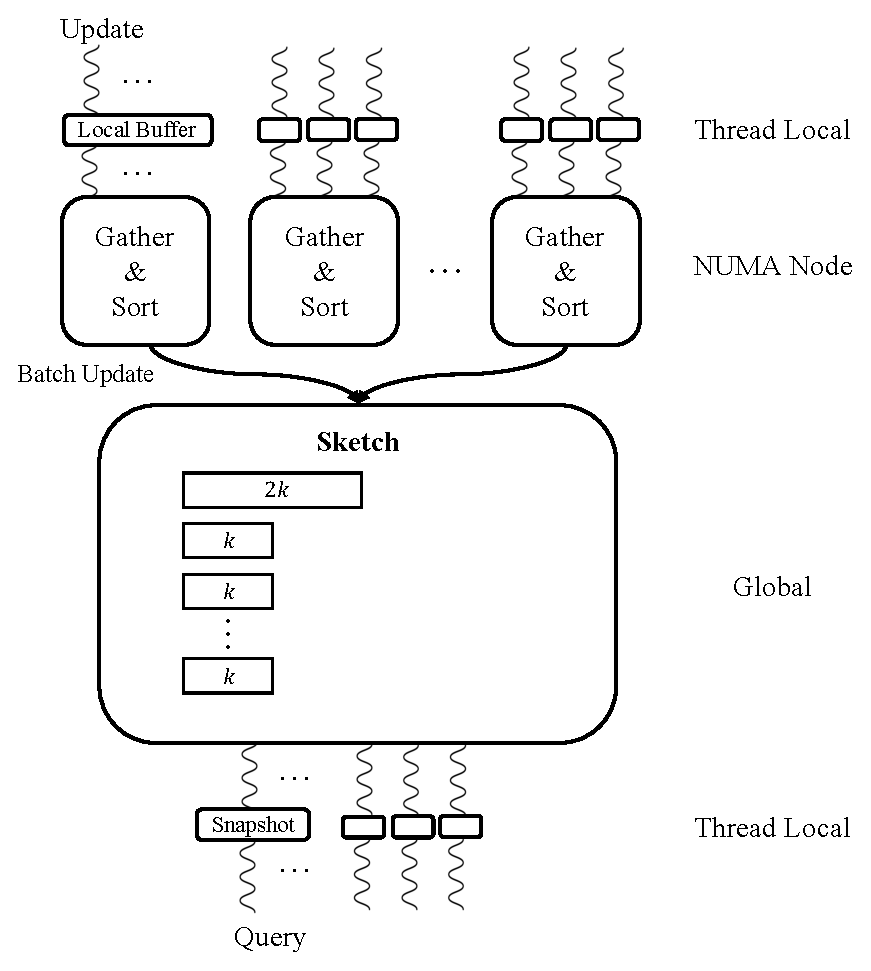
\includegraphics[width=0.8\linewidth,trim={0cm 0cm 0cm 0.1cm},clip]{graphics/algorithm/architecture.pdf}
    \caption{\mysketch's architecture.}
    \label{fig:quancurrentDS}
\end{figure}

% For scalability purposes, queries are served from a cached snapshot of the sketch. How up-to-date the query estimation depends on the sizes of the local and shared buffers and on the freshness of the cached snapshot, both of which are controlled by parameters.

To lower synchronization overhead, we allow buffered elements to be sporadically overwritten by others without being propagated, and others to be duplicated, i.e., propagated more than once. These occurrences, which we call \emph{holes}, alter the stream ingested by the data structure. 
Yet, in Chapter~\ref{chap:analysis} we show that for a sufficiently large local buffer, the expected number of holes is less than $1$ and because they are random, they do not change the sampled distribution.


Figure~\ref{fig:intro-query-accuracy} presents quantiles estimated by \mysketch on a stream of normally distributed random values compared to an exact, brute-force computation of the quantiles, and shows that the estimation is very accurate.

\begin{figure}[htp]
    \centering
    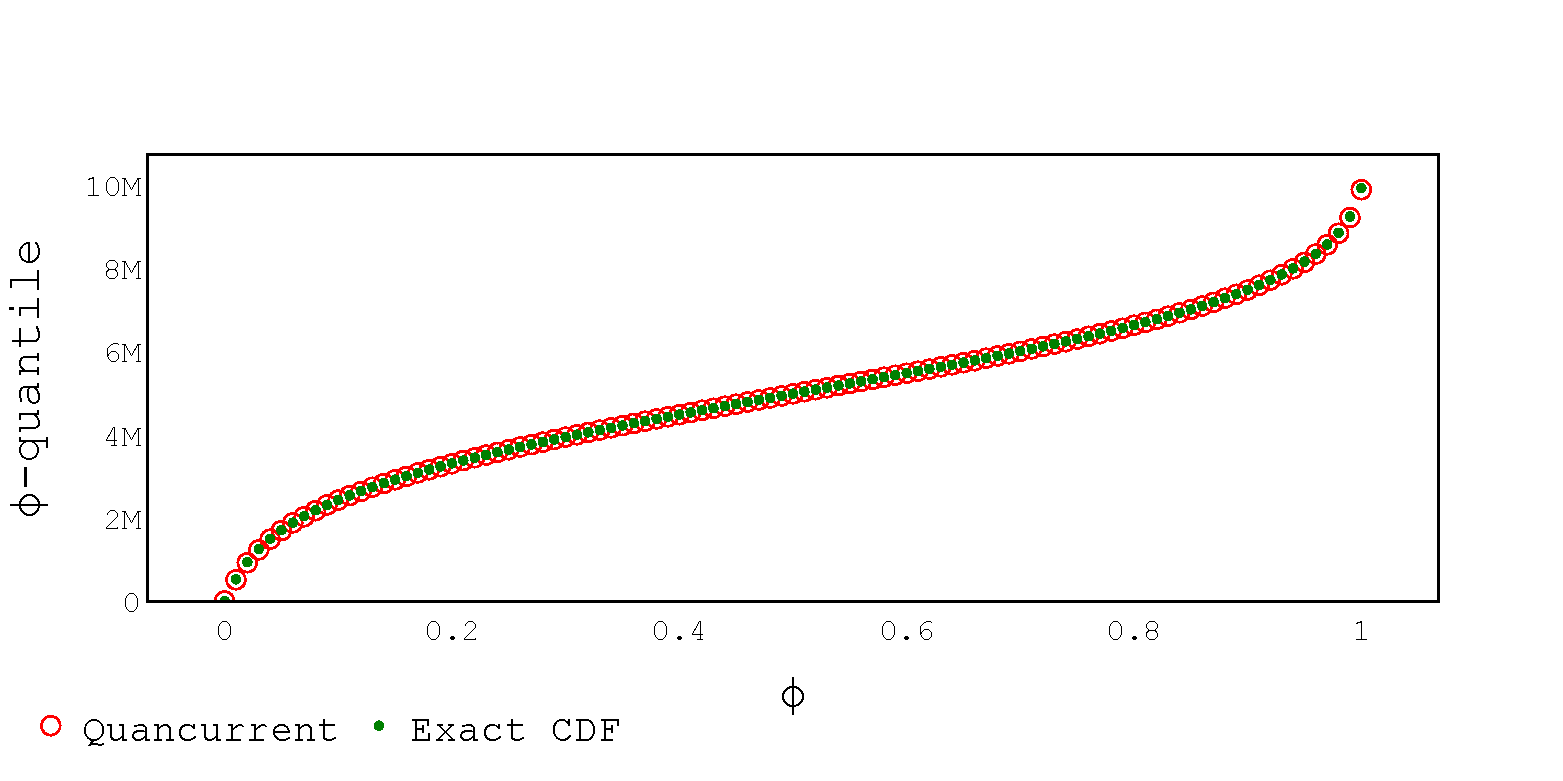
\includegraphics[width=\linewidth,trim={0cm 0.3cm 0cm 1.5cm},clip]
    {graphics/graphs/accuracy/Oracle_Quancurrent_blocking_numa_cdf_normal_k1024_b16_keys10M_runs1_uT32_qT1_snapshot1_17-09-2022_07-00-49.pdf}
    \caption{\mysketch's $\phi$-quantiles vs. exact quantiles (normal distribution, $k=1024$, $32$ update threads, $10M$ elements).}
    \label{fig:intro-query-accuracy}
\end{figure}


In Chapter~\ref{chap:eval} we empirically evaluate \mysketch. We show an update speedup of $12$x and a query speedup of $30$x over the sequential sketch, both with linear speedup. We compare \mysketch to FCDS, which is state-of-the-art in concurrent sketches. We show that for FCDS to achieve similar performance it requires an order of magnitude larger buffers than \mysketch, reducing query freshness tenfold.

In Chapter~\ref{chap:correctness} we present a formal correctness proof. Finally, Chapter~\ref{chap:conclusion} concludes our work and presents some open questions for future research. 


\section{Summary of Contributions} 
We present \mysketch, a scalable Quantiles sketch that retains a small error bound with reasonable query freshness. The main technical challenges we address are:
\begin{enumerate}
  \item High scalability. \mysketch's throughput increases linearly with the number of available threads. High throughput can be achieved with much smaller buffers (hence better query freshness).
  \item Accurate estimates (small error bound, fresh query). \mysketch allows queries to occur concurrently with updates and achieves better query freshness than existing scalable solutions. 
  \item Eliminating sequential propagation bottleneck. \mysketch allows more concurrency than previous solutions by utilizing multiple buffers and allowing multiple threads to concurrently engage in merge-sorts, which are a sequential bottleneck in previous solutions. 
  \item Minimizing synchronization. We leverage the fact that sketches are approximate to begin with to dramatically reduce the synchronization overhead.
  \item Correctness semantics with guaranteed error bounds. \mysketch query's snapshot is strongly linearizable with respect to an r-relaxed sequential Quantiles sketch with \(r=4kS + (N-S)b\).
\end{enumerate}




%
% and then cover:
% - The methods used in the research
% - The research results
% - Discussion and conclusions from the results
%
% but not necessarily with a specific chapter for each of them.
%
% Then you have your main chapters (although these might still
% include an initial chapter on technical preliminaries, experimental
% system setup, and/or a final chapter with summary, discussion and further
% research direction or questions)

\chapter{Preliminaries}
\label{chap:prelims}

We consider a shared memory model, where a finite number of threads execute \emph{operations} on shared \emph{objects}. An operation consists of an \emph{invocation} and a matching \emph{response}. A \emph{history} \(\mathnormal{H}\) is a finite sequence of operation invocation and response steps. A history \(\mathnormal{H}\) defines a partial order \(\prec_\mathnormal{H}\) on operations: Given operations \(op\) and \(op'\), \(op \prec_H op'\) if and only if \(response(op)\) precedes \(invocation(op')\) in \(\mathnormal{H}\). Two operations that do not precede each other are \emph{concurrent}. In a \emph{sequential history}, there are no concurrent operations. An object is specified using a \emph{sequential specification} $\mathcal{H}$, which is the set of its allowed sequential histories.
An operation \emph{op} is \emph{complete} in a history \(\mathnormal{H}\) if both \(invocation(op)\) and its matching \(response(op)\) are in \(\mathnormal{H}\).
A \emph{linearization} of a concurrent history \(\mathnormal{H}\), is a sequential history $H'$ such that: (1) $H' \in \mathcal{H}$, (2) $H'$ contains all completed operations and possibly additional non-complete ones, after adding matching responses, and, (3) $\prec_{H'}$ extends $\prec_H$. A correctness condition for randomized algorithms \emph{strong linearizability}~\cite{strong_linearizability}, defined as follows: 

\begin{definition}[strong linearizability]
\label{def:strong_linearizability}
A function \(f\) mapping executions to histories is \emph{prefix-preserving} if for any two executions $\sigma$, $\sigma$', where $\sigma$ is a prefix of $\sigma$', $f(\sigma)$ is a prefix of $f(\sigma')$. 
An object A is \emph{strongly linearizable} if there is a prefix-preserving function \(f\) that maps every history \(\mathnormal{H}\) of $A$ to a linearization of \(\mathnormal{H}\).
\end{definition}

Our algorithm is randomised and we consider a weak adversary that determines the scheduling without observing the coin-flips.

As previously mentioned, we adopt a flavor of \emph{relaxed semantics}, as defined in \cite{Henzinger_2013_Quantitative_Relaxation}:

\begin{definition}[$r$-relaxation] \label{def:r-relaxtion}
A sequential history $H$ is an \emph{$r$-relaxation} of a sequential history H', if H is comprised of all but at most $r$ of the invocations in $H'$ and their responses,
and each invocation in $H$ is preceded by all but at most $r$ of the invocations that precede the same invocation in $H'$.
The $r$-relaxation of a sequential specification $\mathcal{H}$ is the set of histories that have $r$-relaxations in $\mathcal{H}$:
\[{H}^r \triangleq \left\{ H' \mid \exists H \in \mathcal{H}: H \text{ is an } r\text{-relaxation of } H'\right\}. \]
\end{definition}

\include{main/mainchap1}
\chapter{Conclusion and open questions}
\label{chap:conclusion}



We presented Quancurrent, a concurrent scalable Quantiles sketch. We have evaluated it and shown it to be linearly scalable for both updates and queries while providing accurate estimates, i.e., retaining a small error bound with reasonable query freshness. Moreover, it achieves higher performance than state-of-the-art concurrent quantiles solutions with better query freshness.

Quancurrent's scalability arises from allowing multiple threads to engage concurrently in merge-sorts, which are a sequential bottleneck in previous solutions. We dramatically reduce the synchronization overhead by accommodating occasional data races that cause samples to be duplicated or dropped, a phenomenon we refer to as holes. This approach leverages the observation that sketches are approximate to begin with, and so the impact of such holes is marginal.

Future work may leverage this observation to achieve high scalability in other sketches or approximation algorithms.

Another direction for future work is using a Quantiles sketch to implement a search index. Index structures are used when fast data access is needed. Such data structures are critical in practical settings, where the large amounts of underlying data is paired with high search volumes and with a high level of concurrency on the hardware side via tens or even hundreds of parallel threads. 

% Range index structures, like B-Trees, return the location of a value within a key sorted set. It is common for the index always to be stored in the main memory, with the data itself sitting on disk.
Indexes have been more memory, cache and/or CPU efficient in the past decades. It is common for the index structure always to be stored in the main memory, with the data itself sitting on disk. The B-Tree is a commonly used index structure, which return the location of a value within a key sorted set. 

Kraska et al.~\cite{case_learned_index} suggested that traditional index structures can be enhanced, or even replaced, with learned models, including deep-learning models, termed \emph{learned indexes}. Continuous function, describing the data distribution, can be used to build more efficient data structures or algorithms. As noted by Kraska et al.~\cite{case_learned_index}, indexes are models. For example, a B-Tree can be considered as a model which takes a key as an input and returns the position of a record within a sorted array. Instead of a B-Tree, they suggested a recursive model index. That is, build a hierarchy of models, where at each stage the model takes the key as an input and based on it picks another model, until the final stage predicts the position.

Quantile sketches can summarize large amounts of data in sub-linear space complexity. Therefore, We can use Quantiles sketches to reduce the memory overhead of an index. Also, Quantiles sketch can be used to approximate the data distribution and optimizing different types of index structures.


%
% Add any appendices here; they must come _before_ the bibliography
%
\appendix
%\noappendicestocpagenum
%\addappheadtotoc
\chapter{Holes Analysis Proofs}
\label{appendix:holes-pi-mono}

To show the bound on the expected number of holes, we present some claims. 
In Section~\ref{sec:holes-analysis} we show in Equation~\ref{eq:pi-i-j} that 
\begin{align*}
\pi_{i,j} \leq \left(\frac{1}{2}\right)^{jb + 2i +1} {{jb+2i} \choose i}.
\end{align*}
Consider the following function:
\begin{align*}
f_1(i) \triangleq \left(\frac{1}{2}\right)^{jb + 2i +1} {{jb+2i} \choose i}.
\end{align*}

\begin{claim}\label{claim:holes-f-1}
$f_1(i)$ is monotonically increasing for $i \in \{0,1,\dots,b-1\}$ and for $j,b \in \mathds{N}$. 
\end{claim}

\begin{proof}
For $b=1$, $i \in {0}$ and the claim is immediate.\\
For $b=2$, $i \in {0,1}$ thus,
\begin{align*}
    f_1(0) &= \left(\frac{1}{2}\right)^{2j+1} \\
    f_1(1) &= \left(\frac{1}{2}\right)^{2j+3} {{2j+2} \choose 1} \\
            &= \left(\frac{1}{2}\right)^{2j+1} \cdot \left(\frac{1}{2}\right)^{2} \cdot (2j+2)\\
            &= f_1(0) \cdot \frac{2j+2}{4} \geq f_1(0) \cdot \frac{2+2}{4} = f_1(0).
\end{align*}
For $b>2$, we show that $f_1(i+1)\geq f_1(i)$ for all $i \in \{0,1,\dots,b-2\}$ and for $j,b \in \mathds{N}$

\begin{align*}
    f_1(i) &= \left(\frac{1}{2}\right)^{jb + 2i +1} {{jb+2i} \choose {i}} \\
    f_1(i+1) &= \left(\frac{1}{2}\right)^{jb + 2i +3} {{jb+2i+2} \choose {i+1}} \\
    &= \left(\frac{1}{2}\right)^{jb + 2i +3} \cdot \frac{(jb+2i+2)!}{(jb+i+1)!\cdot(i+1)!} \\
    &= f_1(i) \cdot \frac{1}{4} \cdot \frac{(jb+2i+2)(jb+2i+1)}{(jb+i+1)(i+1)}
\end{align*}

Consider the following function, 
\begin{align}
    
\end{align}


Consider the following function:
\[g(x) = \frac{1}{4} \cdot \frac{(jb+2x+2)(jb+2x+1)}{(jb+x+1)(x+1)}.\]
It is monotonically decreasing for $0 \leq x \leq b-1$. Consider $g(b-2)$:
\[\frac{1}{4} \cdot \frac{(jb+2b-2)(jb+2b-3)}{(jb+b-1)(b-1)}.\]
Denote this function as $h(j)$.
\[h(1) = \frac{1}{4} \cdot \frac{(3b-2)(3b-3)}{(2b-1)(b-1)} \geq 9/8\]
Furthermore, $h(j)$ is a monotonically increasing function, therefore $h(j) \geq 1$ for all $j \geq 1$.

\end{proof}


% Back Matter
% ------------

% The following command will typeset the bibliography,
% then typeset the Hebrew part of the thesis:
% - Cover page
% - Title page
% - Acknowledgements page
%  (NO table of contents or list of figures in Hebrew)
% - (Extended) abstract (1000-2000 words)
%
% based on information you've provided in the thesis-fields file
% (including the relative paths to your bib files). The Hebrew
% content will be typeset in _reverse_page_order_, i.e. first
% in the file will be the last page of the abstract, and the
% Hebrew cover page will be the last page of the file.
%
\makebackmatter

% The resulting PDF can be printed and taken straight to binding,
% i.e. you do not need to flip any pages anywhere. Of course,
% mind the LaTeX error and warning messages, overfull hboxes etc.

\end{document}

